\begin{figure}[H]
\centering
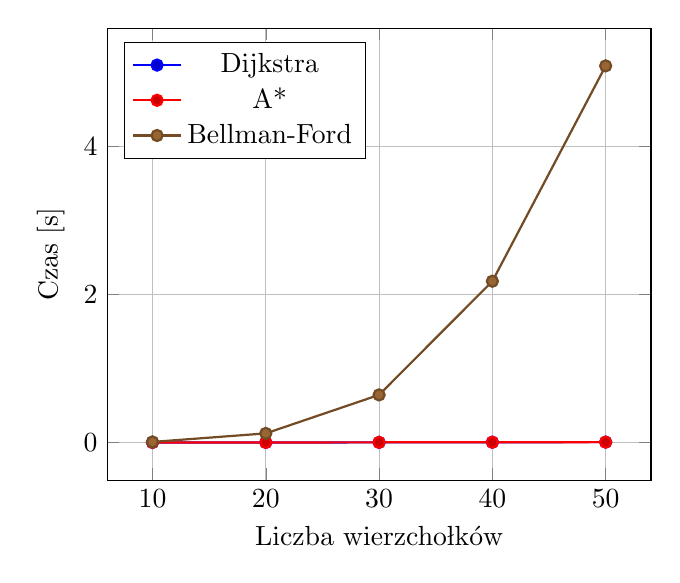
\begin{tikzpicture}
\begin{axis}[
xlabel = {Liczba wierzchołków},
ylabel = {Czas [s]},
legend pos = north west,
grid = both,
width=0.7\linewidth,
]
\addplot + [mark = *, thick] coordinates
    {
(10, 0.00019741058349609375)(20, 0.0006539821624755859)(30, 0.001352071762084961)(40, 0.0037682056427001953)(50, 0.004999399185180664)};
\addlegendentry
{Dijkstra}
\addplot + [mark = *, thick] coordinates
    {
(10, 0.00020766258239746094)(20, 0.0005614757537841797)(30, 0.0016033649444580078)(40, 0.0031180381774902344)(50, 0.004773139953613281)};
\addlegendentry
{A*}
\addplot + [mark = *, thick] coordinates
    {
(10, 0.007578611373901367)(20, 0.12276387214660645)(30, 0.6426141262054443)(40, 2.1777069568634033)(50, 5.085682153701782)};
\addlegendentry
{Bellman-Ford}
\end{axis}
\end{tikzpicture}
\caption
{Porównanie czasów działania algorytmów dla małych instancji}
\label{fig:shortest_path_chart_bellman}
\end{figure}
